\documentclass[aspectratio=169]{beamer}
\useoutertheme[progressbar=frametitle]{metropolis}
\useinnertheme{metropolis}
\definecolor{nabgray}{rgb}{0.6,0.59,0.61}
\usecolortheme[named=nabgray]{structure}
\usepackage{tikz}
\usepackage[utf8]{inputenc}
\usepackage[spanish]{babel}
\usepackage{fontspec}
\setmonofont{JetBrains Mono}
\setmainfont{Roboto}
\setsansfont{Roboto}

\usepackage{smartdiagram}
\usepackage{qtree}
\usepackage{verbatim}
\usepackage{svg}
\usepackage{graphicx}
\usepackage{color}
\definecolor{lightgray}{rgb}{0.95, 0.95, 0.95}
\definecolor{darkgray}{rgb}{0.4, 0.4, 0.4}
\definecolor{ocherCode}{rgb}{1, 0.5, 0} % #FF7F00 -> rgb(239, 169, 0)
\definecolor{blueCode}{rgb}{0, 0, 0.93} % #0000EE -> rgb(0, 0, 238)
\definecolor{greenCode}{rgb}{0, 0.6, 0} % #009900 -> rgb(0, 153, 0) 

\usepackage{upquote}
\usepackage{listings}
\lstset{language=java,
    otherkeywords={var,record},
	% Basic design
	backgroundcolor=\color{lightgray},
	basicstyle={\small\ttfamily},   
	frame=l,
	keywordstyle=\footnotesize\color{blue},
	escapeinside={<@}{@>},
	breaklines=true,
	% Line numbers
	xleftmargin={0.75cm},
	numbers=left,
	stepnumber=1,
	firstnumber=1,
	numberfirstline=true
	% Code design
	identifierstyle=\color{black},
	keywordstyle=\color{ocherCode}\bfseries,
	ndkeywordstyle=\color{greenCode}\bfseries,
	stringstyle=\color{ocherCode}\ttfamily,
	commentstyle=\color{darkgray}\ttfamily,
	tabsize=2,
	showtabs=true,
	showspaces=false,
	showstringspaces=false,
	extendedchars=true,
	breaklines=true
}

\lstdefinelanguage{bash}{
    basicstyle=\ttfamily,
    showstringspaces=false,
    commentstyle=\color{red},
    keywordstyle=\color{blue},
    numbers=right,
    xleftmargin={0.25cm}
}

\usebackgroundtemplate
{
	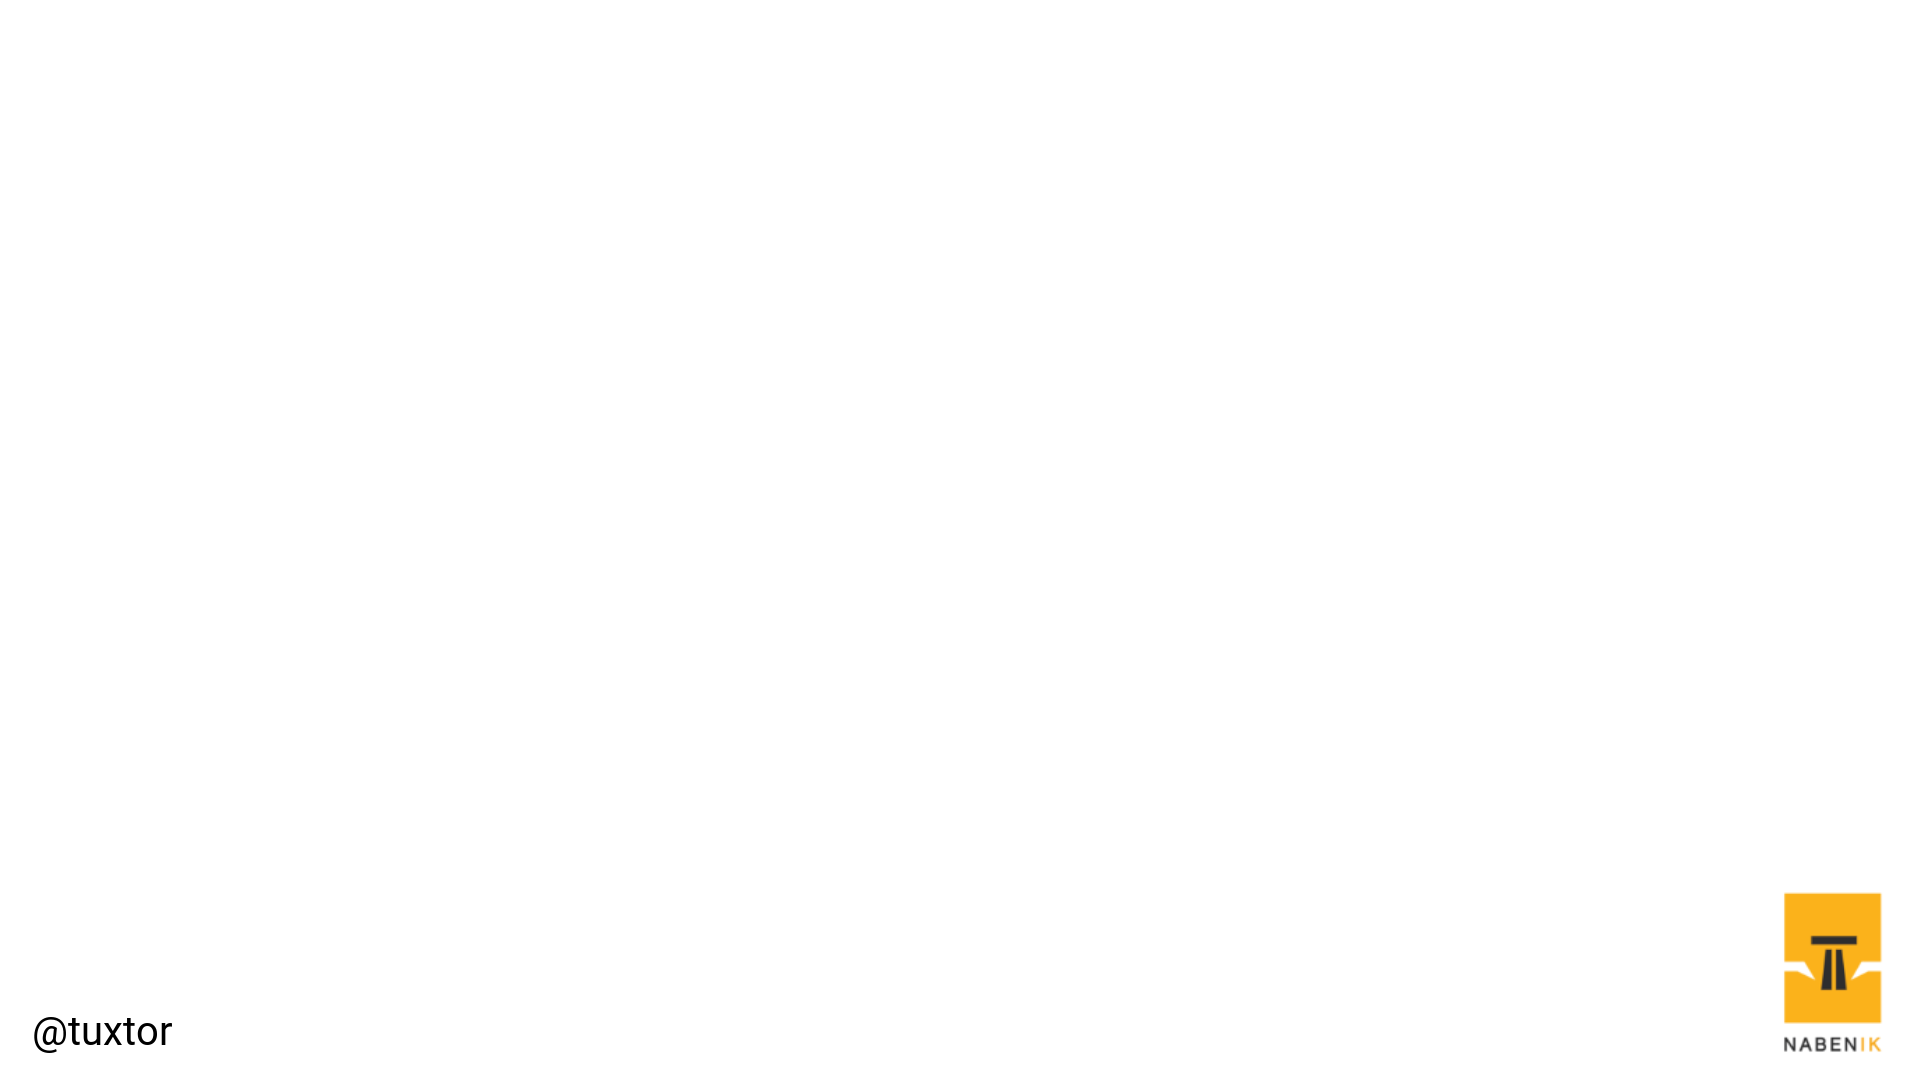
\includegraphics[width=\paperwidth]{Images/fondo}%
}


\title{De Java 8 a Java 14}
\author{Víctor Orozco - @tuxtor}
\institute{Academik}
\date{\today}

\begin{document}

{
    \usebackgroundtemplate{
\includegraphics[width=\paperwidth]{Images/portada}}
    \setbeamercolor{frametitle}{fg=red}
    \usebeamercolor[fg]{normal text}
    \frame{\titlepage}
}


\begin{frame}
    \tableofcontents
\end{frame}

\begin{frame}[fragile]

    \begin{figure}
        \centering
        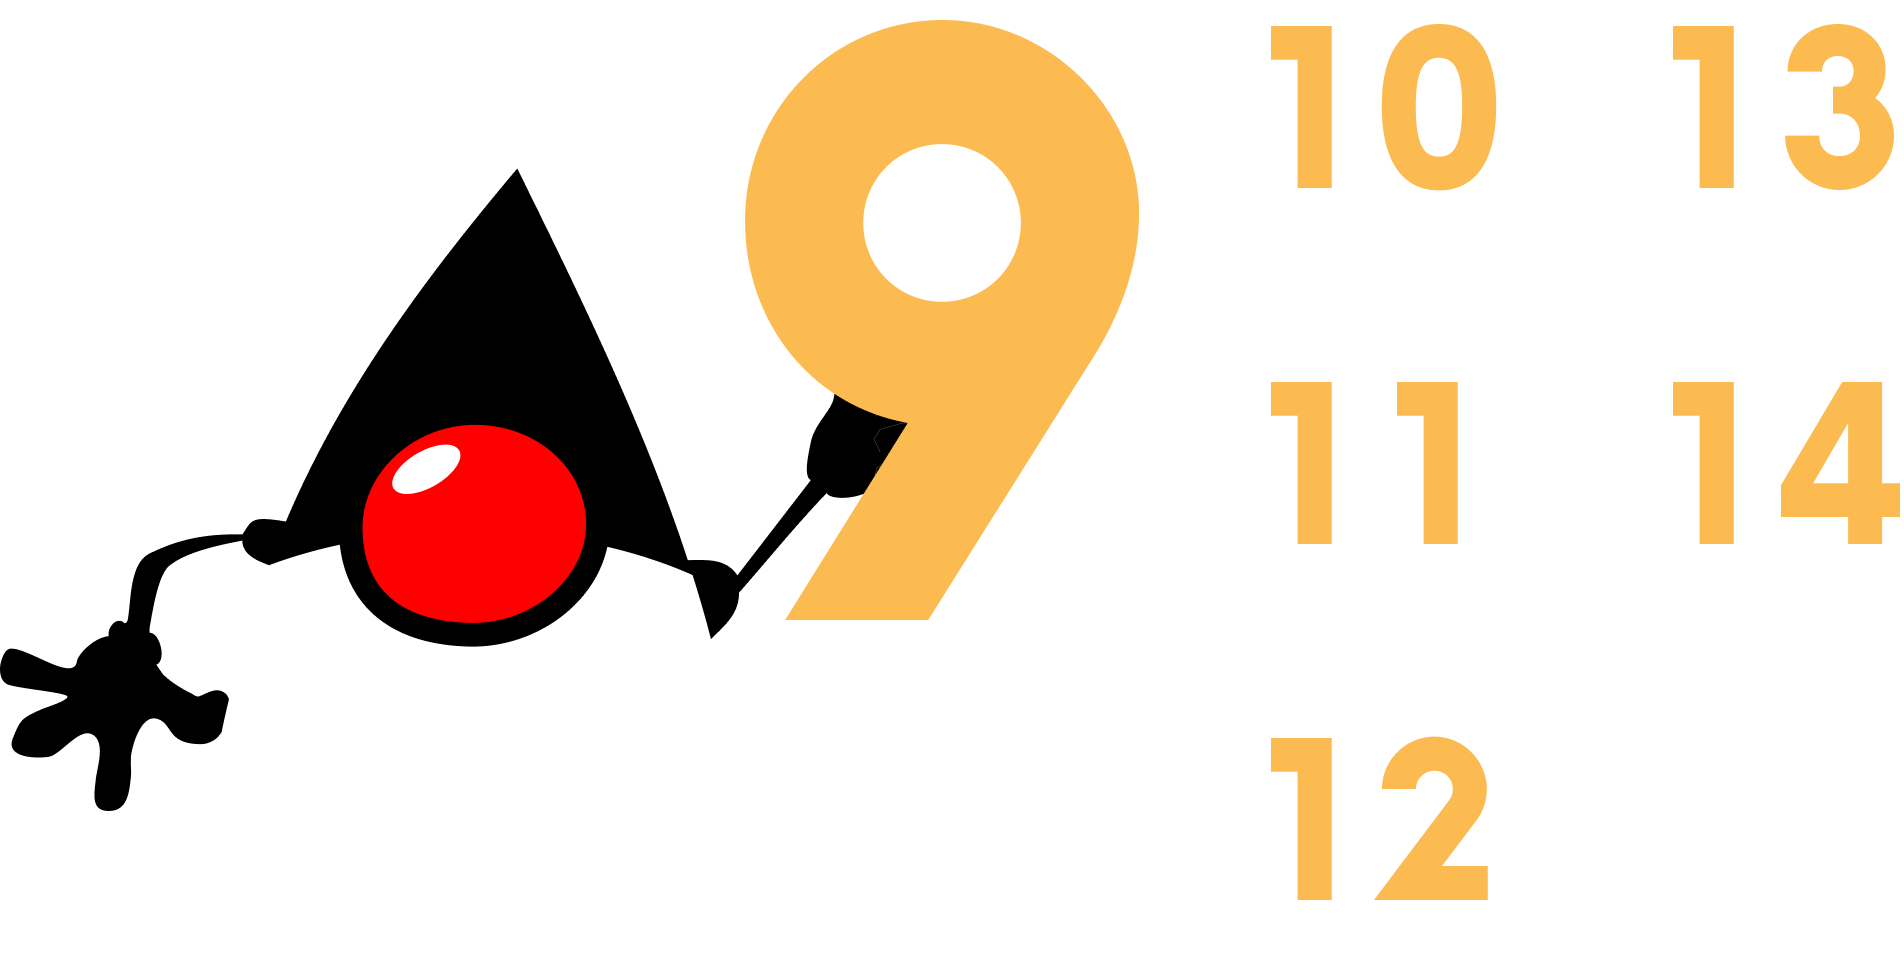
\includegraphics[width=\linewidth]{Images/versiones}
    \end{figure}

\end{frame}

\section{¿Java ya no es gratis/libre?}

\begin{frame}[fragile]{¿Que es Java?}
	\begin{itemize}
		\item Lenguaje de programación
		\item Maquina virtual
		\item Bibliotecas/API
	\end{itemize}

Todas conforman la plataforma Java \pause(TM)
	
\end{frame}

\begin{frame}[fragile]{¿Como se hace Java?}
	\begin{itemize}
		\item JCP - Java Community Process
		\item JSR - Java Specification Request
		\item JEP - Java Enhancement Proposal
		\item JCK - Java Compatibility Kit
	\end{itemize}	
\end{frame}


\begin{frame}[fragile]{¿Como se hace Java? - Java Specification Request}
	\begin{figure}
		\centering
		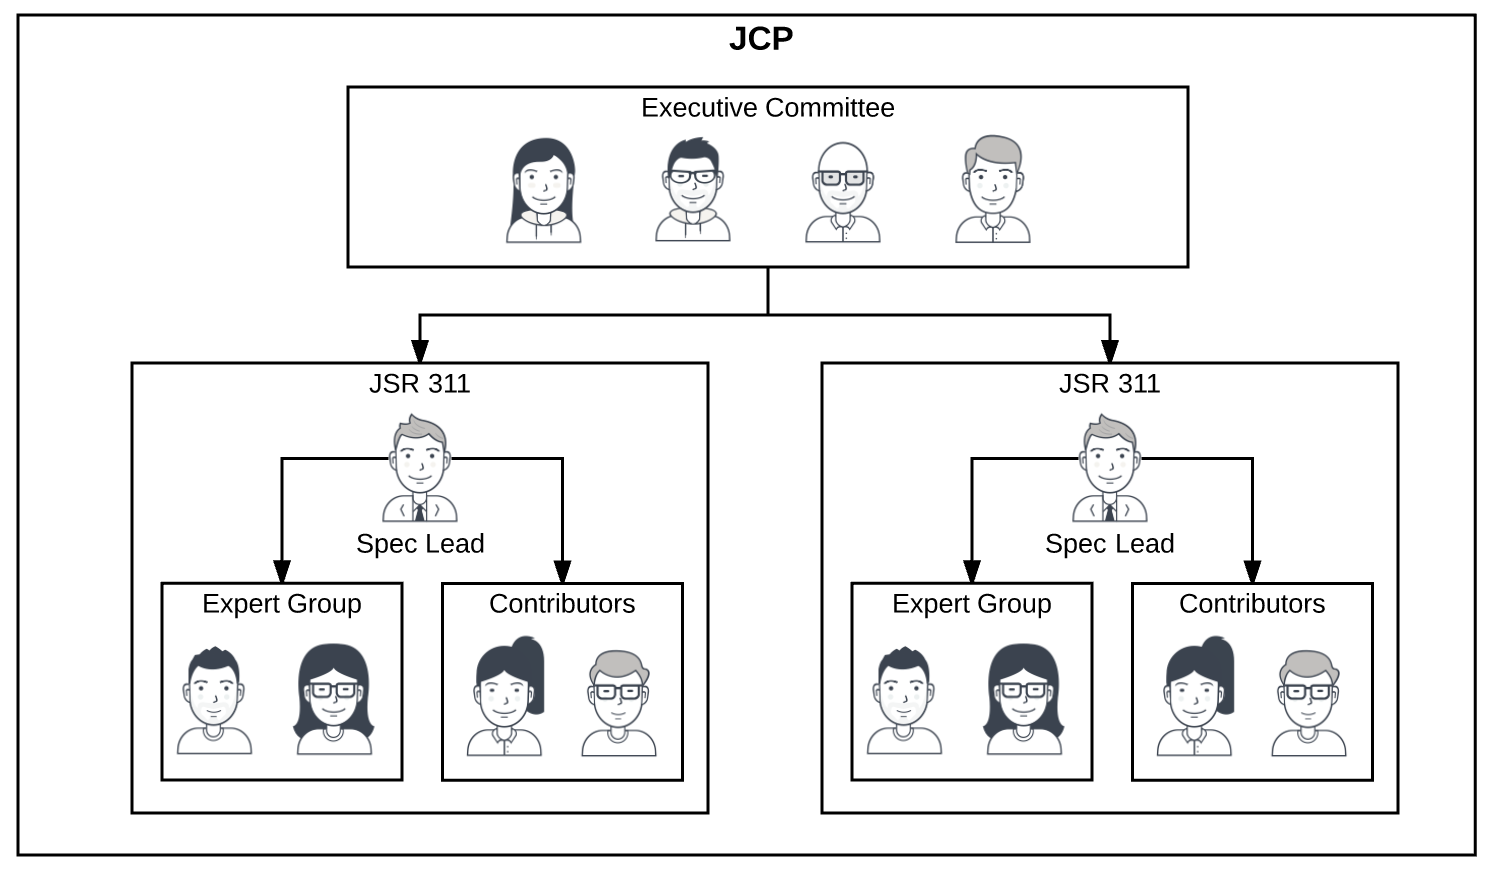
\includegraphics[width=0.9\linewidth]{Images/jcpjsr}
	\end{figure}

\end{frame}

\begin{frame}[fragile]{¿Como se hace Java? - Java Enhancement Proposal}
	\begin{figure}
		\centering
		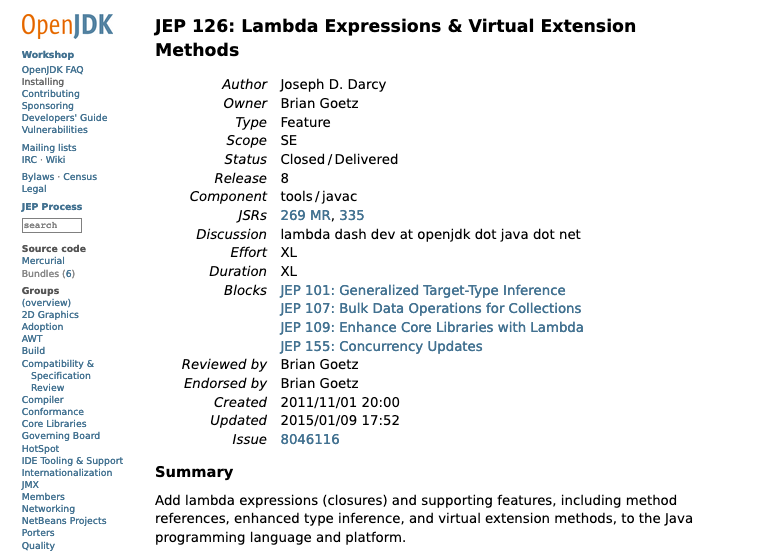
\includegraphics[width=0.9\linewidth]{Images/jep}
	\end{figure}
	
\end{frame}

\begin{frame}[fragile]{¿Como se hace Java? - Java Compatibility Kit}
	\begin{figure}
		\centering
		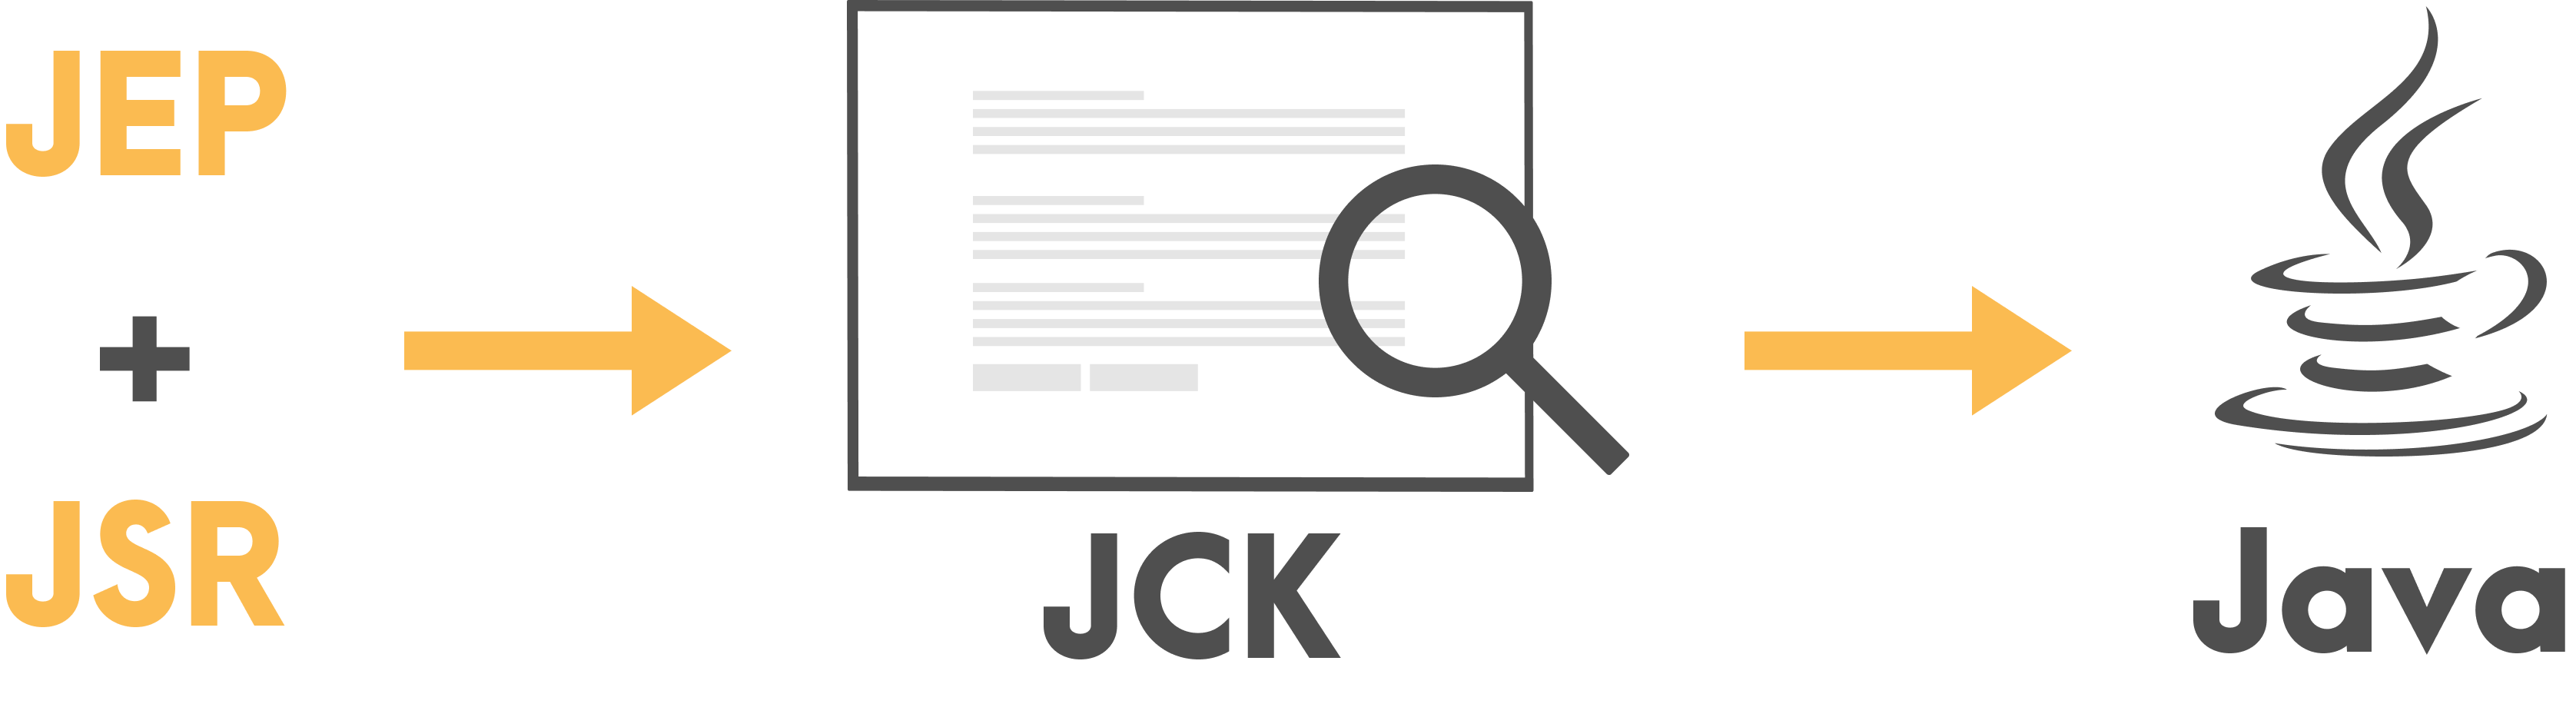
\includegraphics[width=0.9\linewidth]{Images/jck}
	\end{figure}
	
\end{frame}

\begin{frame}[fragile]{¿Como se hace Java? - Java Builds}
	\begin{figure}
		\centering
		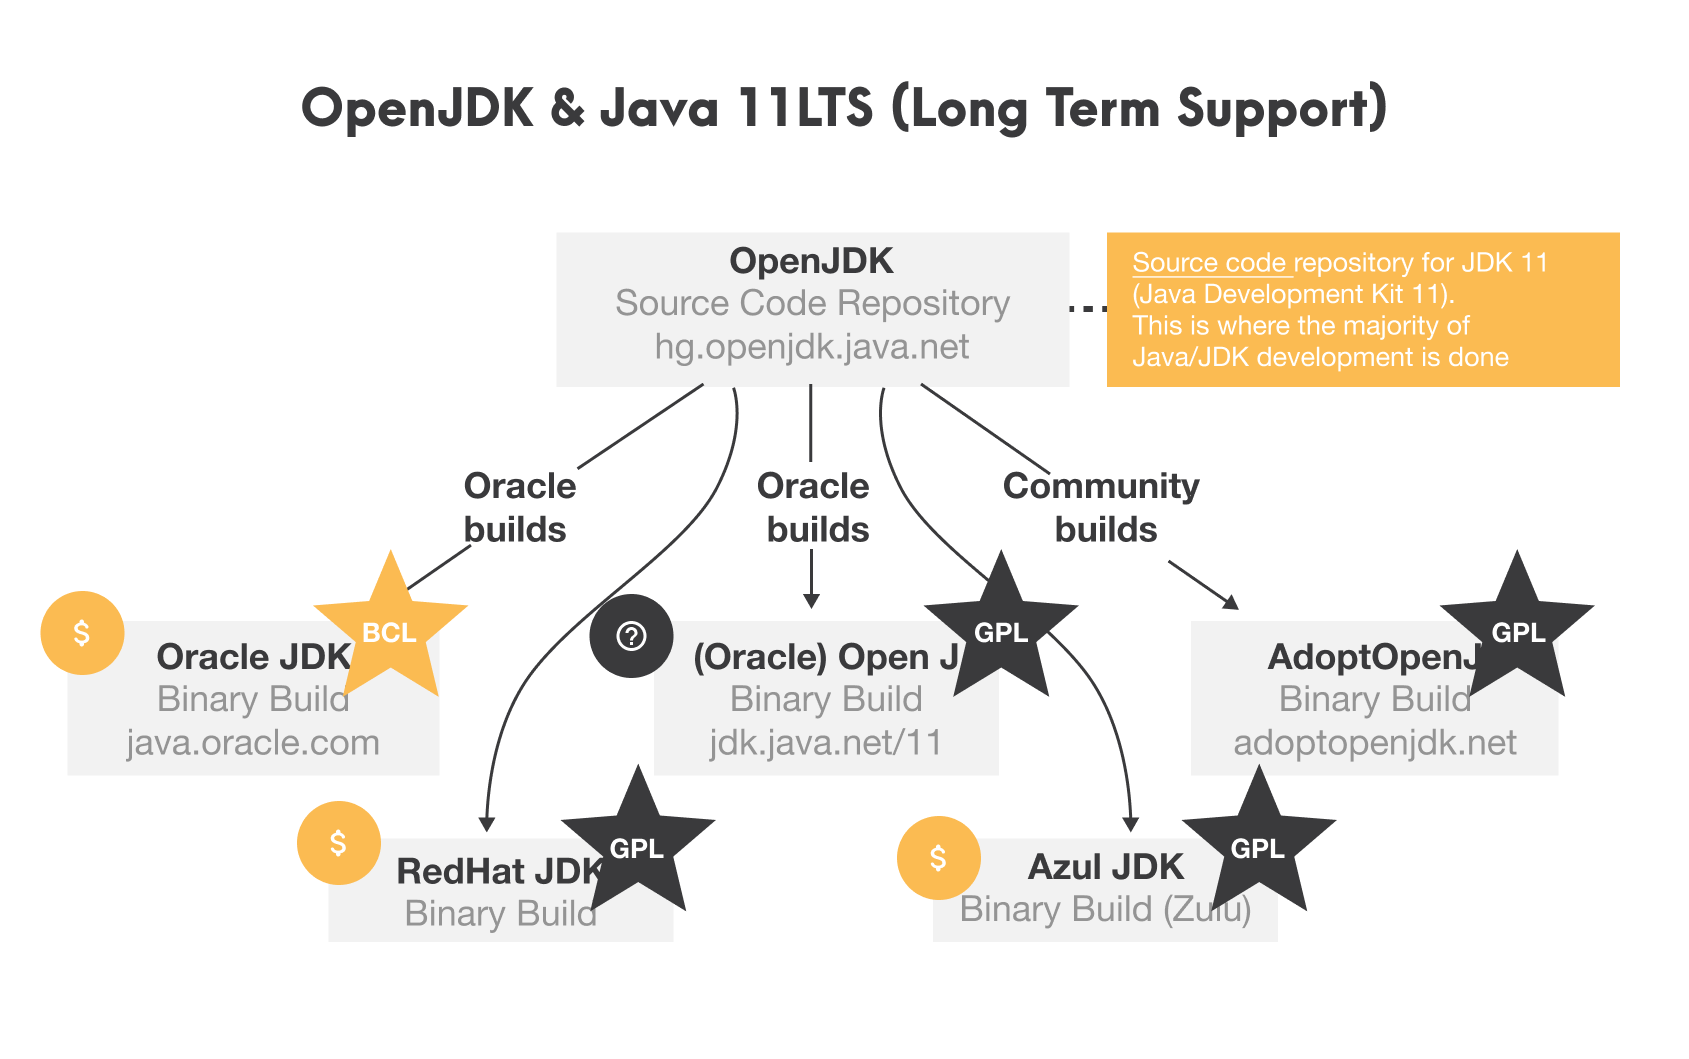
\includegraphics[width=0.9\linewidth]{Images/javabuilds}
	\end{figure}
	
\end{frame}

\begin{frame}[fragile]{¿Java ya no es gratis/libre?}
Java \textbf{es gratis y libre}.

Algunas empresas cobran por soporte en su "versión" de Java.
\end{frame}

{
    \usebackgroundtemplate{
\includegraphics[width=\paperwidth]{Images/separador}}
    \setbeamercolor{normal text}{fg=white}
    \setbeamercolor{frametitle}{fg=red}
    \usebeamercolor[fg]{normal text}
    \section{De Java 8 a Java 14}
}


%TODO Timeline

\begin{frame}[fragile]{¿Una nueva versión de Java?}
	\begin{itemize}
		\item Java - \textbf{Lenguaje de programación}
		\item Java - La plataforma (Bibliotecas y APIs)
		\item Java - La máquina virtual
	\end{itemize}	
\end{frame}



\begin{frame}[fragile]{Java - Mejoras importantes}
	\begin{columns}[T] % contents are top vertically aligned
		
		\begin{column}[T]{5cm} % alternative top-align that's better for graphics
			\begin{itemize}
				\item Java 9
				\begin{itemize}
					\item Modulos
					\item JShell
					\item HTTP/2
                    \item Factory methods
				\end{itemize}
				\item Java 10
				\begin{itemize}
					\item Inferencia de tipos
					\item Class Data Sharing
					\item Time based release
				\end{itemize}
			\end{itemize}
		\end{column}
		\begin{column}[T]{5cm} % each column can also be its own environment
			\begin{itemize}
                \item Java 11
                \begin{itemize}
                    \item String methods
                    \item File methods
                    \item Ejecución directa de .java
                \end{itemize}
				\item Java 12
				\begin{itemize}
					\item Switch expressions
				\end{itemize}
				\item Java 13
				\begin{itemize}
					\item Text blocks
				\end{itemize}
				\item Java 14
				\begin{itemize}
					\item Pattern matching
					\item Records
					\item Helpfull NPE
				\end{itemize}
			\end{itemize}
		\end{column}
	\end{columns}
\end{frame}

{
    \usebackgroundtemplate{
\includegraphics[width=\paperwidth]{Images/separador}}
    \setbeamercolor{normal text}{fg=white}
    \setbeamercolor{frametitle}{fg=red}
    \usebeamercolor[fg]{normal text}
    \section{Java 9}
}



\begin{frame}[fragile]{JEP 222: jshell: The Java Shell (Read-Eval-Print Loop)}
    \begin{figure}
        \centering
        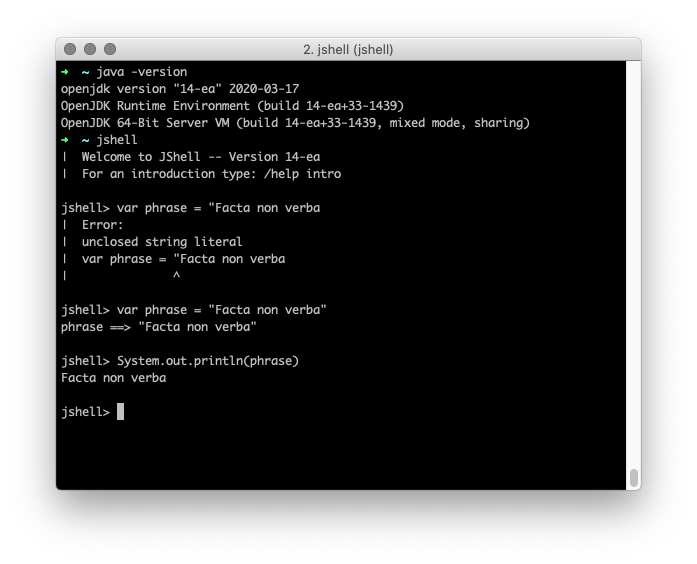
\includegraphics[width=0.9\linewidth]{Images/jshell}
    \end{figure}
    
\end{frame}

\begin{frame}[fragile]{JEP 110: HTTP/2 Client }
\begin{lstlisting}
HttpRequest request = HttpRequest.newBuilder()
    .uri(new URI("https://swapi.co/api/starships/9"))
    .GET()
    .build();

HttpResponse<String> response = HttpClient.newHttpClient()
    .send(request, BodyHandlers.ofString());
    
System.out.println(response.body());
\end{lstlisting}
\end{frame}


\begin{frame}[fragile]{JEP 269: Convenience Factory Methods for Collections}
Antes
\begin{lstlisting}
Set<String> set = new HashSet<>();
set.add("a");
set.add("b");
set.add("c");
set = Collections.unmodifiableSet(set);
\end{lstlisting}	

"Pro"
\begin{lstlisting}
Set<String> set = Collections.unmodifiableSet(new HashSet<>(Arrays.asList("a", "b", "c")));
\end{lstlisting}	

Ahora
\begin{lstlisting}
Set<String> set = Set.of("a", "b", "c");
\end{lstlisting}
\end{frame}


\begin{frame}[fragile]{JEP 213: Milling Project Coin - Private methods in interfaces}
Antes
\begin{lstlisting}
public interface Vehicle{
    public void move();
}
\end{lstlisting}	

Ahora
\begin{lstlisting}[basicstyle=\scriptsize]
public interface Vehicle{
    public default void makeNoise(){
        System.out.println("Making noise!");
        createNoise();
    }

    private void createNoise(){
        System.out.println("Run run");
    } 
}
\end{lstlisting}	
    
\end{frame}

\begin{frame}[fragile]{JEP 213: Milling Project Coin - Try-with-resources}
Antes
\begin{lstlisting}
BufferedReader reader = new BufferedReader(new FileReader("langs.txt"));

try(BufferedReader innerReader = reader){
    System.out.println(reader.readLine());
}
\end{lstlisting}	

Ahora
\begin{lstlisting}
BufferedReader reader = new BufferedReader(new FileReader("langs.txt"));

try(reader){
    System.out.println(reader.readLine());
}
\end{lstlisting}	
    
\end{frame}

{
    \usebackgroundtemplate{
\includegraphics[width=\paperwidth]{Images/separador}}
    \setbeamercolor{normal text}{fg=white}
    \setbeamercolor{frametitle}{fg=red}
    \usebeamercolor[fg]{normal text}
    \section{Java 10}
}


\begin{frame}[fragile]{Java 10}
\textbf{286: Local-Variable Type Inference}\\
296: Consolidate the JDK Forest into a Single Repository\\
304: Garbage-Collector Interface\\
307: Parallel Full GC for G1\\
\textbf{310: Application Class-Data Sharing}\\
312: Thread-Local Handshakes\\
313: Remove the Native-Header Generation Tool (javah)\\
314: Additional Unicode Language-Tag Extensions\\
316: Heap Allocation on Alternative Memory Devices\\
317: Experimental Java-Based JIT Compiler\\
319: Root Certificates\\
\textbf{322: Time-Based Release Versioning}\\
\end{frame}

\begin{frame}[fragile]{JEP 286: Local-Variable Type Inference}
\begin{lstlisting}
public static void main(String args[]){
    var localValue = 99;
    System.out.println(++localValue);
    //localValue = "Foo"
}
\end{lstlisting}	
\end{frame}



\begin{frame}[fragile]{JEP 310: Application Class-Data Sharing}
\begin{lstlisting}[language=bash,basicstyle=\scriptsize]
java -XX:ArchiveClassesAtExit=app-cs.jsa -jar payara-micro-5.192.jar
java -XX:SharedArchiveFile=app-cs.jsa -jar fpjava.jar
\end{lstlisting}	
\end{frame}
\begin{frame}[fragile]{JEP 310: Application Class-Data Sharing}
    \begin{figure}
        \centering
        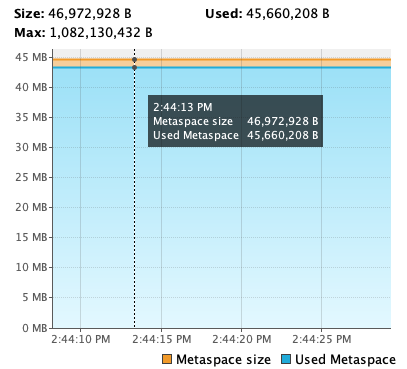
\includegraphics[width=0.7\linewidth]{Images/nocdsmem}
    \end{figure}
\end{frame}
\begin{frame}[fragile]{JEP 310: Application Class-Data Sharing}
    \begin{figure}
        \centering
        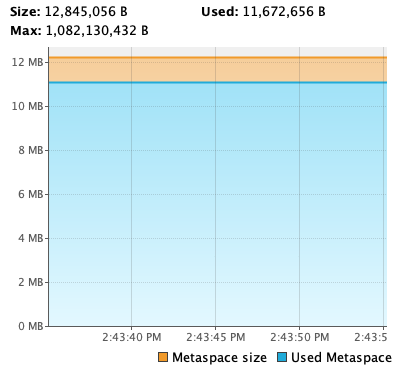
\includegraphics[width=0.7\linewidth]{Images/cdsmem}
    \end{figure}
\end{frame}


\begin{frame}[fragile]{JEP 322: Time-Based Release Versioning}
    \begin{figure}
        \centering
        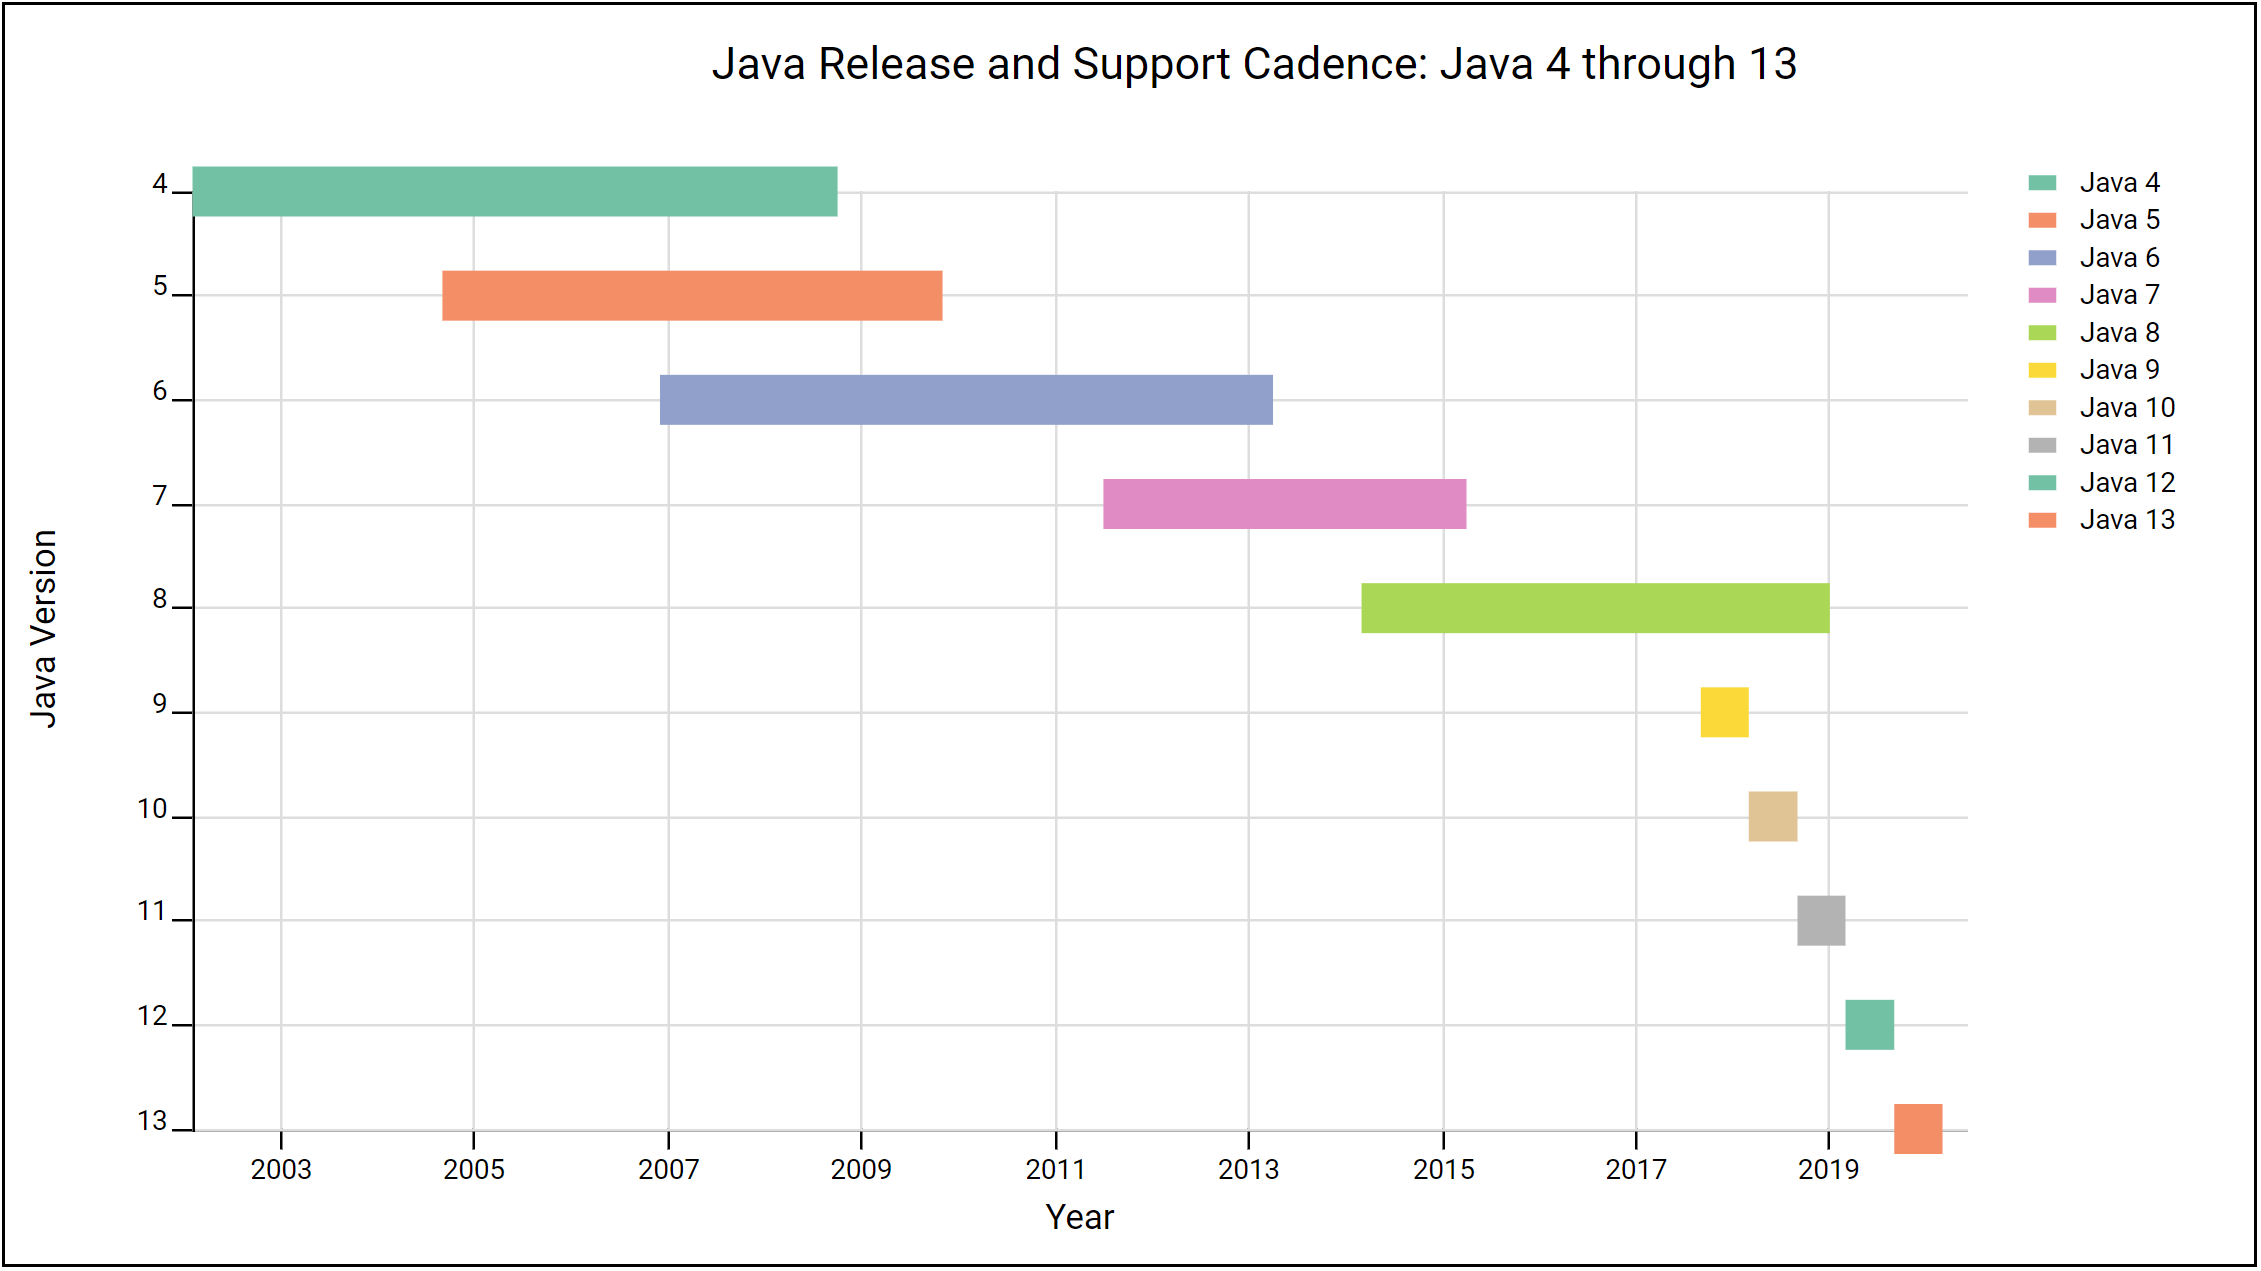
\includegraphics[width=0.9\linewidth]{Images/javacadence}
    \end{figure}
\end{frame}
   
\begin{frame}[fragile]{JEP 322: Time-Based Release Versioning}
    \begin{figure}
        \centering
        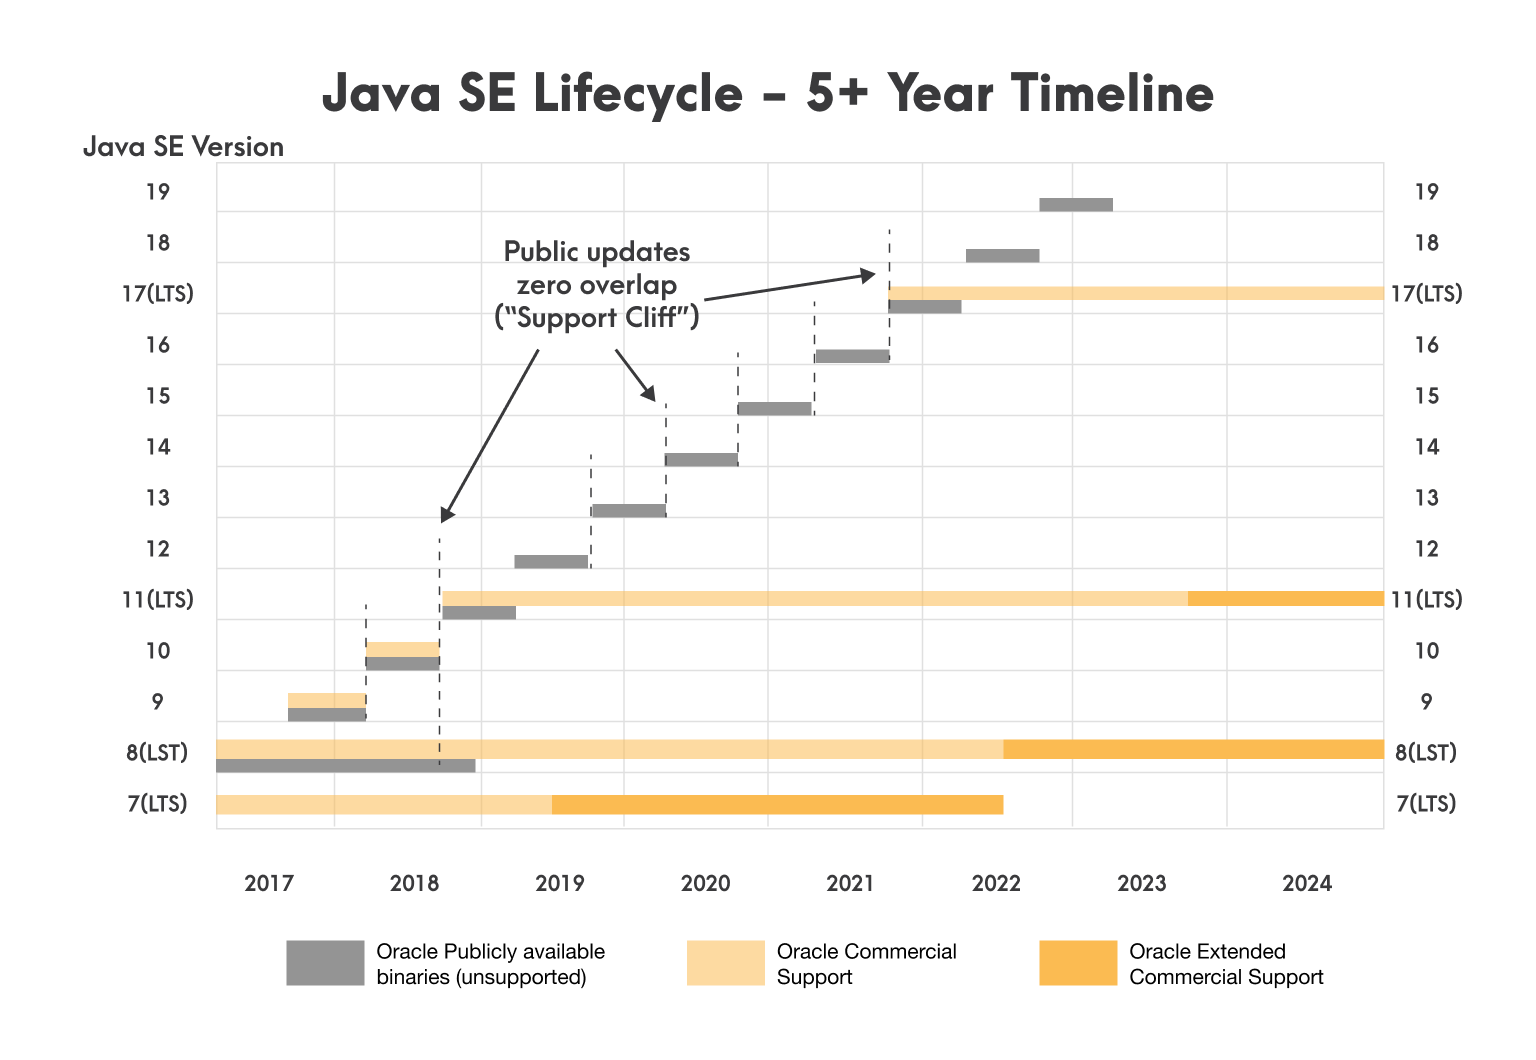
\includegraphics[width=0.9\linewidth]{Images/javarelease}
    \end{figure}
\end{frame}

{
    \usebackgroundtemplate{
\includegraphics[width=\paperwidth]{Images/separador}}
    \setbeamercolor{normal text}{fg=white}
    \setbeamercolor{frametitle}{fg=red}
    \usebeamercolor[fg]{normal text}
    \section{Java 11}
}

\begin{frame}[fragile]{Java 11}\scriptsize
\begin{columns}[T] % contents are top vertically aligned
    
    \begin{column}[T]{6cm} % alternative top-align that's better for graphics
        181: Nest-Based Access Control\\
        309: Dynamic Class-File Constants\\
        315: Improve Aarch64 Intrinsics\\
        318: Epsilon: A No-Op Garbage Collector\\
        \textbf{320: Remove the Java EE and CORBA Modules}\\
        321: HTTP Client (Standard)\\
        \textbf{323: Local-Variable Syntax for Lambda Parameters}\\
        324: Key Agreement with Curve25519 and Curve448\\
        327: Unicode 10\\
        328: Flight Recorder\\
    \end{column}
    \begin{column}[T]{6cm} % each column can also be its own environment
        329: ChaCha20 and Poly1305 Cryptographic Algorithms\\
        \textbf{330: Launch Single-File Source-Code Programs}\\
        331: Low-Overhead Heap Profiling\\
        332: Transport Layer Security (TLS) 1.3\\
        333: ZGC: A Scalable Low-Latency Garbage Collector
        (Experimental)\\
        \textbf{335: Deprecate the Nashorn JavaScript Engine}\\
        336: Deprecate the Pack200 Tools and API\\
    \end{column}
\end{columns}
\end{frame}
    

\begin{frame}[fragile]{JEP 323: Local-Variable Syntax for Lambda Parameters}
Antes
\begin{lstlisting}
BiPredicate<String,String> demoPredicate =
    (String a, String b) -> a.equals(b);
BiPredicate<String,String> demoPredicate =
    (a, b) -> a.equals(b);
\end{lstlisting}

Ahora
\begin{lstlisting}
BiPredicate<String,String> demoPredicate =
    (var a, var b) -> a.equals(b);
\end{lstlisting}	

Posibilidades
\begin{lstlisting}
(@Nonnull var x, @Nullable var y) -> x.process(y)
\end{lstlisting}	
\end{frame}

\begin{frame}[fragile]{JEP 330: Launch Single-File Source-Code Programs}
    \begin{figure}
        \centering
        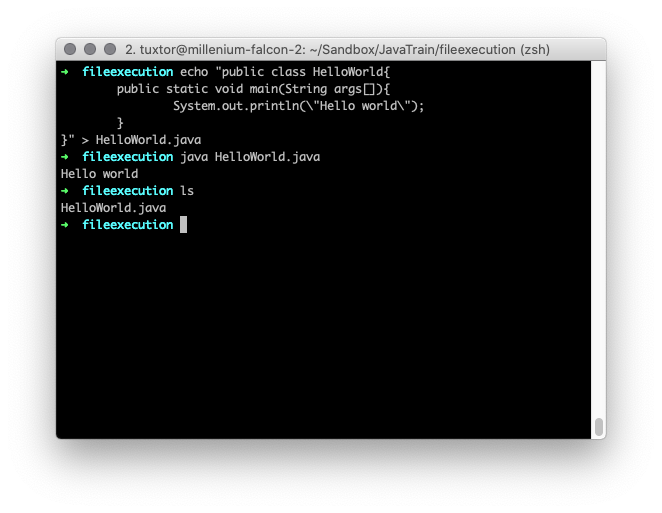
\includegraphics[width=0.9\linewidth]{Images/jep222singlefile}
    \end{figure}
    
\end{frame}

{
    \usebackgroundtemplate{
\includegraphics[width=\paperwidth]{Images/separador}}
    \setbeamercolor{normal text}{fg=white}
    \setbeamercolor{frametitle}{fg=red}
    \usebeamercolor[fg]{normal text}
    \section{Java 12}
}



\begin{frame}[fragile]{Java 12}
189: Shenandoah: A Low-Pause-Time Garbage Collector (Experimental)\\
230: Microbenchmark Suite\\
\textbf{325: Switch Expressions (Preview)}\\
334: JVM Constants API\\
340: One AArch64 Port, Not Two\\
341: Default CDS Archives\\
344: Abortable Mixed Collections for G1\\
346: Promptly Return Unused Committed Memory from G1
\end{frame}


\begin{frame}[fragile]{325: Switch Expressions (Preview)}
Antes
\begin{lstlisting}
String langType = "";
switch (args[0]) {
    case "Java":
    case "Scala":
    case "Kotlin":
        langType = "Static typed";
        break;
    case "Groovy":
    case "JavaScript":
        langType = "Dynamic typed";
        break;
}
System.out.println(langType);
\end{lstlisting}	
\end{frame}

\begin{frame}[fragile]{325: Switch Expressions (Preview)}
Ahora
\begin{lstlisting}
String langType = switch (args[0]) {
    case "Java", "Scala", "Kotlin" -> "Static typed";
    case "Groovy", "JavaScript" -> "Dynamic typed";
    default -> {
        System.out.println("This meant to be a processing block");
        yield "Probably LISP :)";
    }
};
System.out.println(langType);
\end{lstlisting}	
\end{frame}

{
    \usebackgroundtemplate{
\includegraphics[width=\paperwidth]{Images/separador}}
    \setbeamercolor{normal text}{fg=white}
    \setbeamercolor{frametitle}{fg=red}
    \usebeamercolor[fg]{normal text}
    \section{Java 13}
}

\begin{frame}[fragile]{Java 13}
350: Dynamic CDS Archives\\
351: ZGC: Uncommit Unused Memory\\
353: Reimplement the Legacy Socket API\\
354: \textbf{Switch Expressions (Preview)}\\
355: \textbf{Text Blocks (Preview)}\\
\end{frame}

\begin{frame}[fragile]{355: Text Blocks (Preview)}
Antes
\begin{lstlisting}
String html = "<html>\n" +
"    <body>\n" +
"        <p>Hello, world</p>\n" +
"    </body>\n" +
"</html>\n";
\end{lstlisting}

Ahora
\begin{lstlisting}
String html = """
<html>
    <body>
        <p>Hello, world</p>
    </body>
</html>
""";
\end{lstlisting}
\end{frame}

{
    \usebackgroundtemplate{
\includegraphics[width=\paperwidth]{Images/separador}}
    \setbeamercolor{normal text}{fg=white}
    \setbeamercolor{frametitle}{fg=red}
    \usebeamercolor[fg]{normal text}
    \section{Java 14}
}
\begin{frame}[fragile]{Java 14}\scriptsize
    \begin{columns}[T] % contents are top vertically aligned
        
        \begin{column}[T]{6cm} % alternative top-align that's better for graphics
            \textbf{305: Pattern Matching for instanceof (Preview)}\\
            343: Packaging Tool (Incubator)\\
            345: NUMA-Aware Memory Allocation for G1\\
            349: JFR Event Streaming\\
            352: Non-Volatile Mapped Byte Buffers\\
            \textbf{358: Helpful NullPointerExceptions}\\
            \textbf{359: Records (Preview)}\\
            \textbf{361: Switch Expressions (Standard)}
        \end{column}
        \begin{column}[T]{6cm} % each column can also be its own environment
            362: Deprecate the Solaris and SPARC Ports\\
            363: Remove the Concurrent Mark Sweep (CMS) Garbage Collector\\
            364: ZGC on macOS\\
            365: ZGC on Windows\\
            366: Deprecate the ParallelScavenge + SerialOld GC Combination\\
            367: Remove the Pack200 Tools and API\\
            368: Text Blocks (Second Preview)\\
            370: Foreign-Memory Access API (Incubator)
        \end{column}
    \end{columns}
\end{frame}

\begin{frame}[fragile]{JEP 359: Records (Preview)}
Data carrier
\begin{lstlisting}
record Person(String name, String email, int age) {}
\end{lstlisting}

Uso
\begin{lstlisting}
Person foo = new Person("Marco", "example@mail.com",99);
System.out.println(foo);
//foo.name = "Polo";
\end{lstlisting}	
\end{frame}

\begin{frame}[fragile]{305:	Pattern Matching for instanceof (Preview)}
Antes
\begin{lstlisting}
if(o instanceof Person){
    Person p = (Person)o;
    System.out.println("Hello " + p.name());
}else{
    System.out.println("Unknown object");
}
\end{lstlisting}	

Ahora
\begin{lstlisting}
if(o instanceof Person p){
    System.out.println("Hello " + p.name());
}else{
    System.out.println("Unknown object");
}
\end{lstlisting}	
\end{frame}

{
    \usebackgroundtemplate{
\includegraphics[width=\paperwidth]{Images/separador}}
    \setbeamercolor{normal text}{fg=white}
    \setbeamercolor{frametitle}{fg=red}
    \usebeamercolor[fg]{normal text}
    \section{Mundo real}
}

\begin{frame}[fragile]{Mundo real}\scriptsize
    
Mi mundo real
    \begin{itemize}
        \item ERP - 10 modulos (1 EAR, 9 EJB, 1 WAR), JBoss/Wildfly
        \item Venta/Geocerca (5 WAR) Payara Application Server
        \item POS - JavaFX y Windows D:
    \end{itemize}
Los dolores de cabeza
\begin{itemize}
    \item Modulos
    \item sun.misc.unsafe
    \item Corba y Java EE
    \item JavaFX
    \item IDE
    \item Licencia
\end{itemize}
\end{frame}

\begin{frame}[fragile]{Mundo real}\scriptsize

    Los dolores de cabeza
    \begin{itemize}
        \item Modulos
        \item sun.misc.unsafe
        \item Corba y Java EE
        \item JavaFX
        \item IDE
        \item Licencia
    \end{itemize}
    
    Estrategia
    \begin{enumerate}
        \item Verificar la compatibilidad del runtime/servidor/framework compatible
        \item Multiples JVM con cambio fácil en desarrollo
        \item Actualizar el compilador en Maven
        \item Actualizar bibliotecas
        \item Incluir los modulos corba y Java EE en el war
        \item Actualizar el IDE
        \item Prepara el proyecto para enlazar el modulo de JavaFX
        \item Verificar que Java necesito
        \item Multiples JVM en producción
    \end{enumerate}
\end{frame}

\begin{frame}[fragile]{Compatibilidad runtime}
    Compatible con Java 11
    \begin{itemize}
        \item Tomcat
        \item Spring
        \item Micronaut
        \item Vert.x
        \item JakartaEE (JBoss/Wildfly, OpenLiberty, Payara)
    \end{itemize}
\end{frame}

\begin{frame}[fragile]{Multiples JVMs}
\begin{columns}[T] % contents are top vertically aligned
    
    \begin{column}[T]{5cm} % alternative top-align that's better for graphics
        \begin{figure}
            \centering
            
\includegraphics[width=\linewidth]{Images/jenv}
        \end{figure}
    \end{column}
    \begin{column}[T]{6cm} % each column can also be its own environment
        \begin{figure}
            \centering
            
\includegraphics[width=\linewidth]{Images/sdkman}
        \end{figure}
    \end{column}
\end{columns}
\end{frame}

\begin{frame}[fragile]{Bibliotecas}
    Manipulación de bytecode
    \begin{itemize}
        \item ByteBuddy
        \item ASM
        \item glib
        \item Spring
        \item Java EE
        \item Hibernate
        \item Mockito
    \end{itemize}
\end{frame}

\begin{frame}[fragile]{Maven}
    \begin{itemize}
        \item Maven 3.5.0
        \item Compiler 3.8.0
        \item surefire 2.22.0
        \item failsafe 2.22.0
        \item release version 11.0
    \end{itemize}
    
\end{frame}

\begin{frame}[fragile]{Maven - JavaEE}
JAF (java.activation)

\begin{lstlisting}[language=xml]
<dependency>
    <groupId>com.sun.activation</groupId>
    <artifactId>javax.activation</artifactId>
    <version>1.2.0</version>
</dependency>
\end{lstlisting}



CORBA = RIP
\end{frame}

\begin{frame}[fragile]{Maven - JavaEE}
JAXB (java.xml.bind)
    
\begin{lstlisting}[language=xml]
<!-- API -->
<dependency>
    <groupId>jakarta.xml.bind</groupId>
    <artifactId>jakarta.xml.bind-api</artifactId>
    <version>2.3.2</version>
</dependency>

<!-- Runtime -->
<dependency>
    <groupId>org.glassfish.jaxb</groupId>
    <artifactId>jaxb-runtime</artifactId>
    <version>2.3.2</version>
</dependency>
\end{lstlisting}
\end{frame}

\begin{frame}[fragile]{Maven - JavaEE}
    JAX-WS (java.xml.ws)
    
\begin{lstlisting}[language=xml]
<!-- API -->
<dependency>
    <groupId>jakarta.xml.ws</groupId>
    <artifactId>jakarta.xml.ws-api</artifactId>
    <version>2.3.2</version>
</dependency>

<!-- Runtime -->
<dependency>
    <groupId>com.sun.xml.ws</groupId>
    <artifactId>jaxws-rt</artifactId>
    <version>2.3.2</version>
</dependency>
\end{lstlisting}
\end{frame}

\begin{frame}[fragile]{Maven - JavaEE}
Common Annotations (java.xml.ws.annotation)

\begin{lstlisting}[language=xml]
<dependency>
    <groupId>javax.annotation</groupId>
    <artifactId>javax.annotation-api</artifactId>
    <version>1.3.1</version>
</dependency>
\end{lstlisting}
\end{frame}

\begin{frame}[fragile]{IDEs}
    
    Compatibles con Java 11
    \begin{itemize}
        \item Eclipse
        \item NetBeans
        \item IntelliJ IDEA
    \end{itemize}
    
    Algunos plugins problematicos
    \begin{enumerate}
        \item Glassfish
        \item WebLogic
        \item Icefaces
    \end{enumerate}
\end{frame}

\begin{frame}[fragile]{JavaFX}
    
    JavaFX ahora es un modulo OpenSource y la forma "recomendada" para empaquetar la aplicación es JPMS, la forma más facil es la compilación de Gluon
    \begin{figure}
        \centering
        
\includegraphics[width=\linewidth]{Images/gluon}
    \end{figure}
\end{frame}

\begin{frame}[fragile]{¿Que Java necesito?}
    Obligatorios por contrato
    \begin{itemize}
        \item Software comercial de Oracle (HotSpot)
        \item Software comercial de SAP (SAP VM)
        \item Software comercial de Red Hat (OpenJDK + RHEL)
        \item Software comercial de IBM (J9)
    \end{itemize}
    Otras opciones
\begin{itemize}
    \item AdoptOpenJDK (Opción a soporte de IBM en J9)
    \item Correto
    \item Azul Zulu
    \item Java de su distro
\end{itemize}
\end{frame}

\begin{frame}[fragile]{Multiples JVMs en producción}
    Linux
    \begin{itemize}
        \item Docker
        \item RHEL
        \item Debian
        \item Gentoo
    \end{itemize}
    Windows
    \begin{itemize}
        \item Docker
        \item Variables de entorno por proyecto/runtime
        \item Lo importante es la salud
    \end{itemize}
\end{frame}


\begin{frame}[fragile]{Academik}
    \begin{columns}[T]
        \begin{column}[T]{2cm} % alternative top-align that's better for graphics
            \begin{figure}
                \centering
                
\includegraphics[width=\linewidth]{Images/qr}
            \end{figure}
        \end{column}
        \begin{column}[T]{12cm} % each column can also be its own environment
        \begin{figure}
            \centering
            
\includegraphics[width=\linewidth]{Images/academik}
        \end{figure}
        \end{column}
    \end{columns}
\end{frame}





\begin{frame}{Víctor Orozco}
\begin{columns}[T] % contents are top vertically aligned
	
	\begin{column}[T]{4cm} % alternative top-align that's better for graphics
		\begin{figure}
			\centering
			
\includegraphics[width=\linewidth]{Images/logos}
		\end{figure}
	\end{column}
	\begin{column}[T]{6cm} % each column can also be its own environment
		\begin{itemize}
			\item vorozco@nabenik.com
			\item \href{https://twitter.com/tuxtor}{@tuxtor}
			\item \href{http://vorozco.com}{http://vorozco.com}
			\item \href{http://tuxtor.shekalug.org}{http://tuxtor.shekalug.org} 
		\end{itemize}
		\begin{center}
			
\includegraphics[width=0.1\linewidth]{Images/cclogo}
			\\
			This work is licensed under Creative Commons Attribution-NonCommercial-ShareAlike 3.0 Guatemala (CC BY-NC-SA 3.0 GT).
		\end{center}
	\end{column}
\end{columns}
\end{frame}

{
    \usebackgroundtemplate{
\includegraphics[width=\paperwidth]{Images/final}}
\begin{frame}
\end{frame}
}

\end{document}

